\documentclass[a4paper]{article}
\usepackage{latexsym}
\usepackage[a4paper]{geometry}
\usepackage{color}
\usepackage{listings}
\usepackage[pdftex]{graphicx}
\usepackage{subfig}
\usepackage{float}

\definecolor{Blue}{rgb}{0,0,0.5}
\definecolor{Green}{rgb}{0,0.75,0.0}
\definecolor{LightGray}{rgb}{0.6,0.6,0.6}
\definecolor{DarkGray}{rgb}{0.3,0.3,0.3}
\lstset{language=Matlab,
   keywords={function,uint8,uint16,uint32,double,break,case,catch,continue,else,elseif,end,for,global,if,otherwise,persistent,return,switch,try,while},
   basicstyle=\ttfamily\small,
   breaklines=true,
   keywordstyle=\bfseries\color{Blue},
   commentstyle=\itshape\color{LightGray},
   stringstyle=\color{Green},
   numbers=left,
   numberstyle=\tiny\color{DarkGray},
   stepnumber=1,
   numbersep=10pt,
   backgroundcolor=\color{white},
   tabsize=2,
   showspaces=false,
   showstringspaces=false,
   captionpos=b}

%Boldface text for type writer font
\usepackage{bold-extra} %\DeclareFontShape{OT1}{cmtt}{bx}{n}{<5><6><7><8><9><10><10.95><12><14.4><17.28><20.74><24.88>cmttb10}{}

%Break words properly at the end of a line (which isn't sloppy...)
\sloppy

%Use command \exercise for each exercise
\newcounter{exerciseCount}
\setcounter{exerciseCount}{0}
\newcommand{\exercise}[1]{\addtocounter{exerciseCount}{1} \noindent \medskip {\large \textsf{\textbf{Exercise \arabic{exerciseCount} \--- #1}}} \par}
\renewcommand{\theenumi}{\textsf{\textbf{\alph{enumi}}}}

%Use command \code for code snippets
\newcommand{\code}[1]{\textnormal{\texttt{#1}}}



\title{\textsf{Image Processing \\ lab 1}}
\author{Klaas Kliffen \and Jan Kramer}
\date{\today}

\begin{document}
\maketitle

\exercise{Zooming and shrinking by pixel replication}
\begin{enumerate}
\item
There are two cases, one for shrinking and zooming.
In case of shrinking we create a new image with the desired dimensions calculated from the factor.
For each pixel in the new image, the corresponding pixel from the original image is sampled.
In the case of zooming, the desired are calculated in a similar fashion.
Instead of sampling, the corresponding pixel from the original is duplicated multiple times.
\lstinputlisting{../lab1ex1/IPresize.m}
\item 
\begin{figure}[H]
\centering
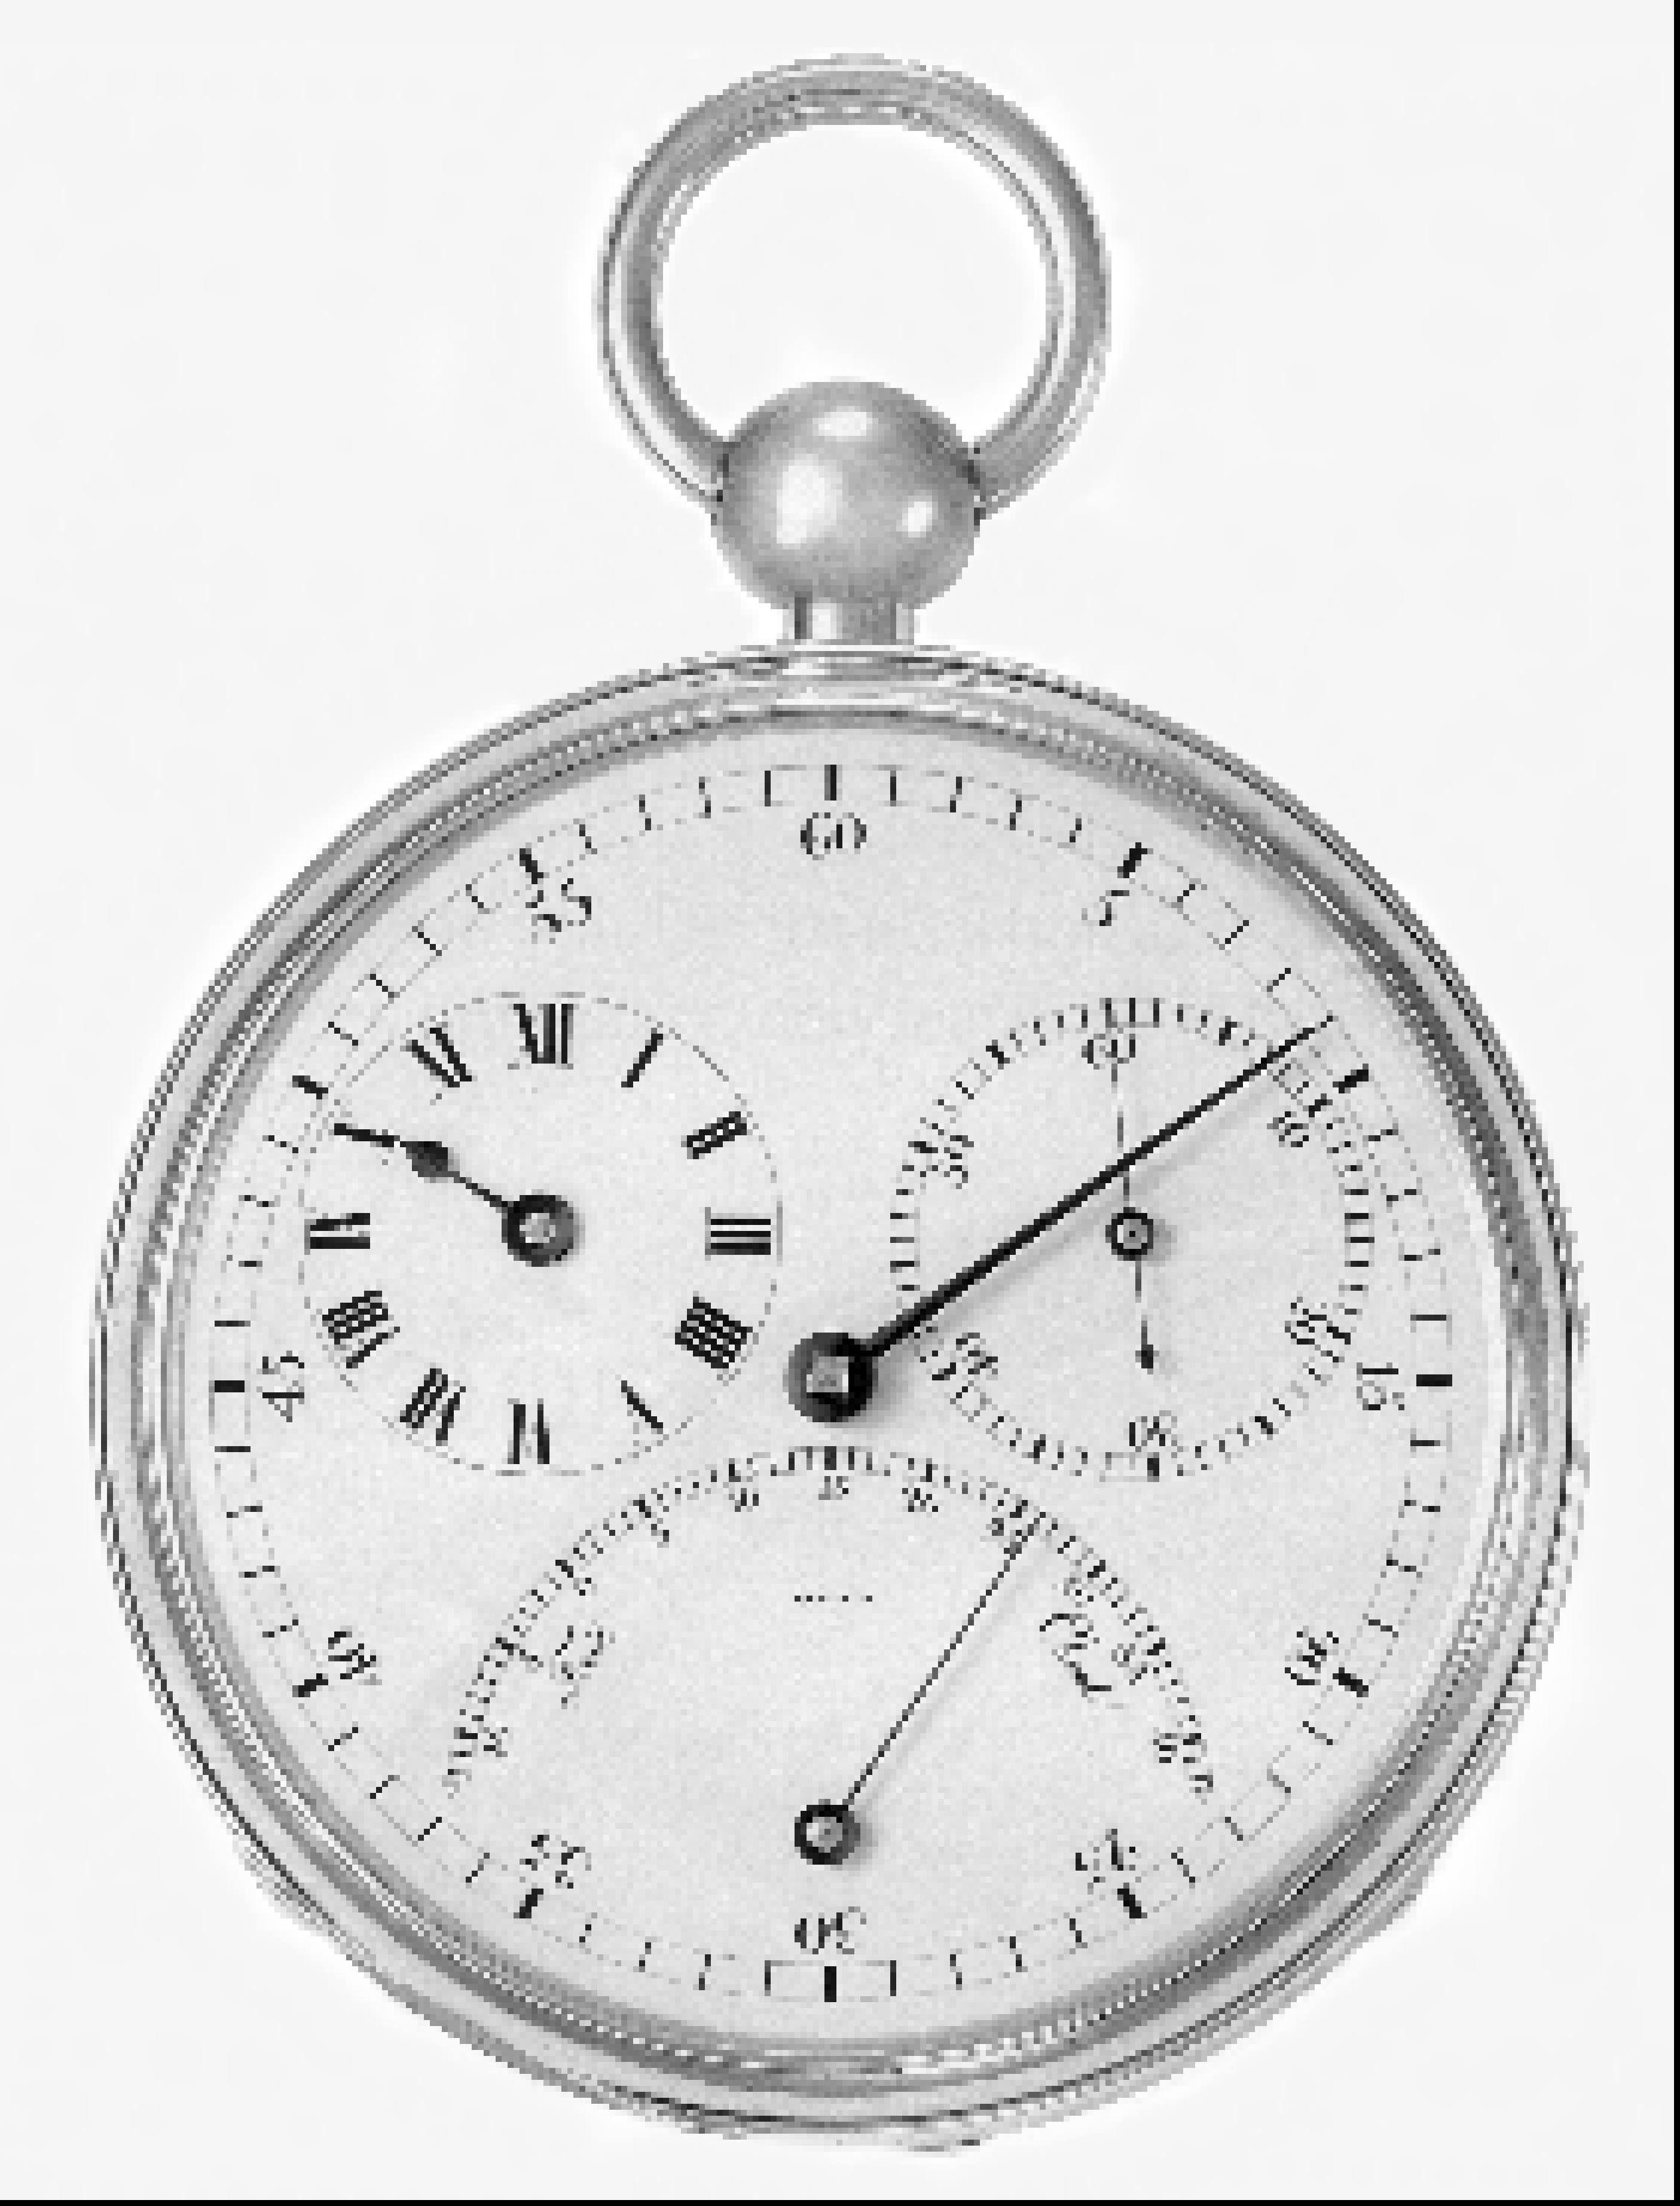
\includegraphics[width=.25\textwidth]{../lab1ex1/clocklow.png}
\caption{The resulting image of shrinking and then zooming with a factor 10}
\end{figure}
\begin{figure}[H]
\centering
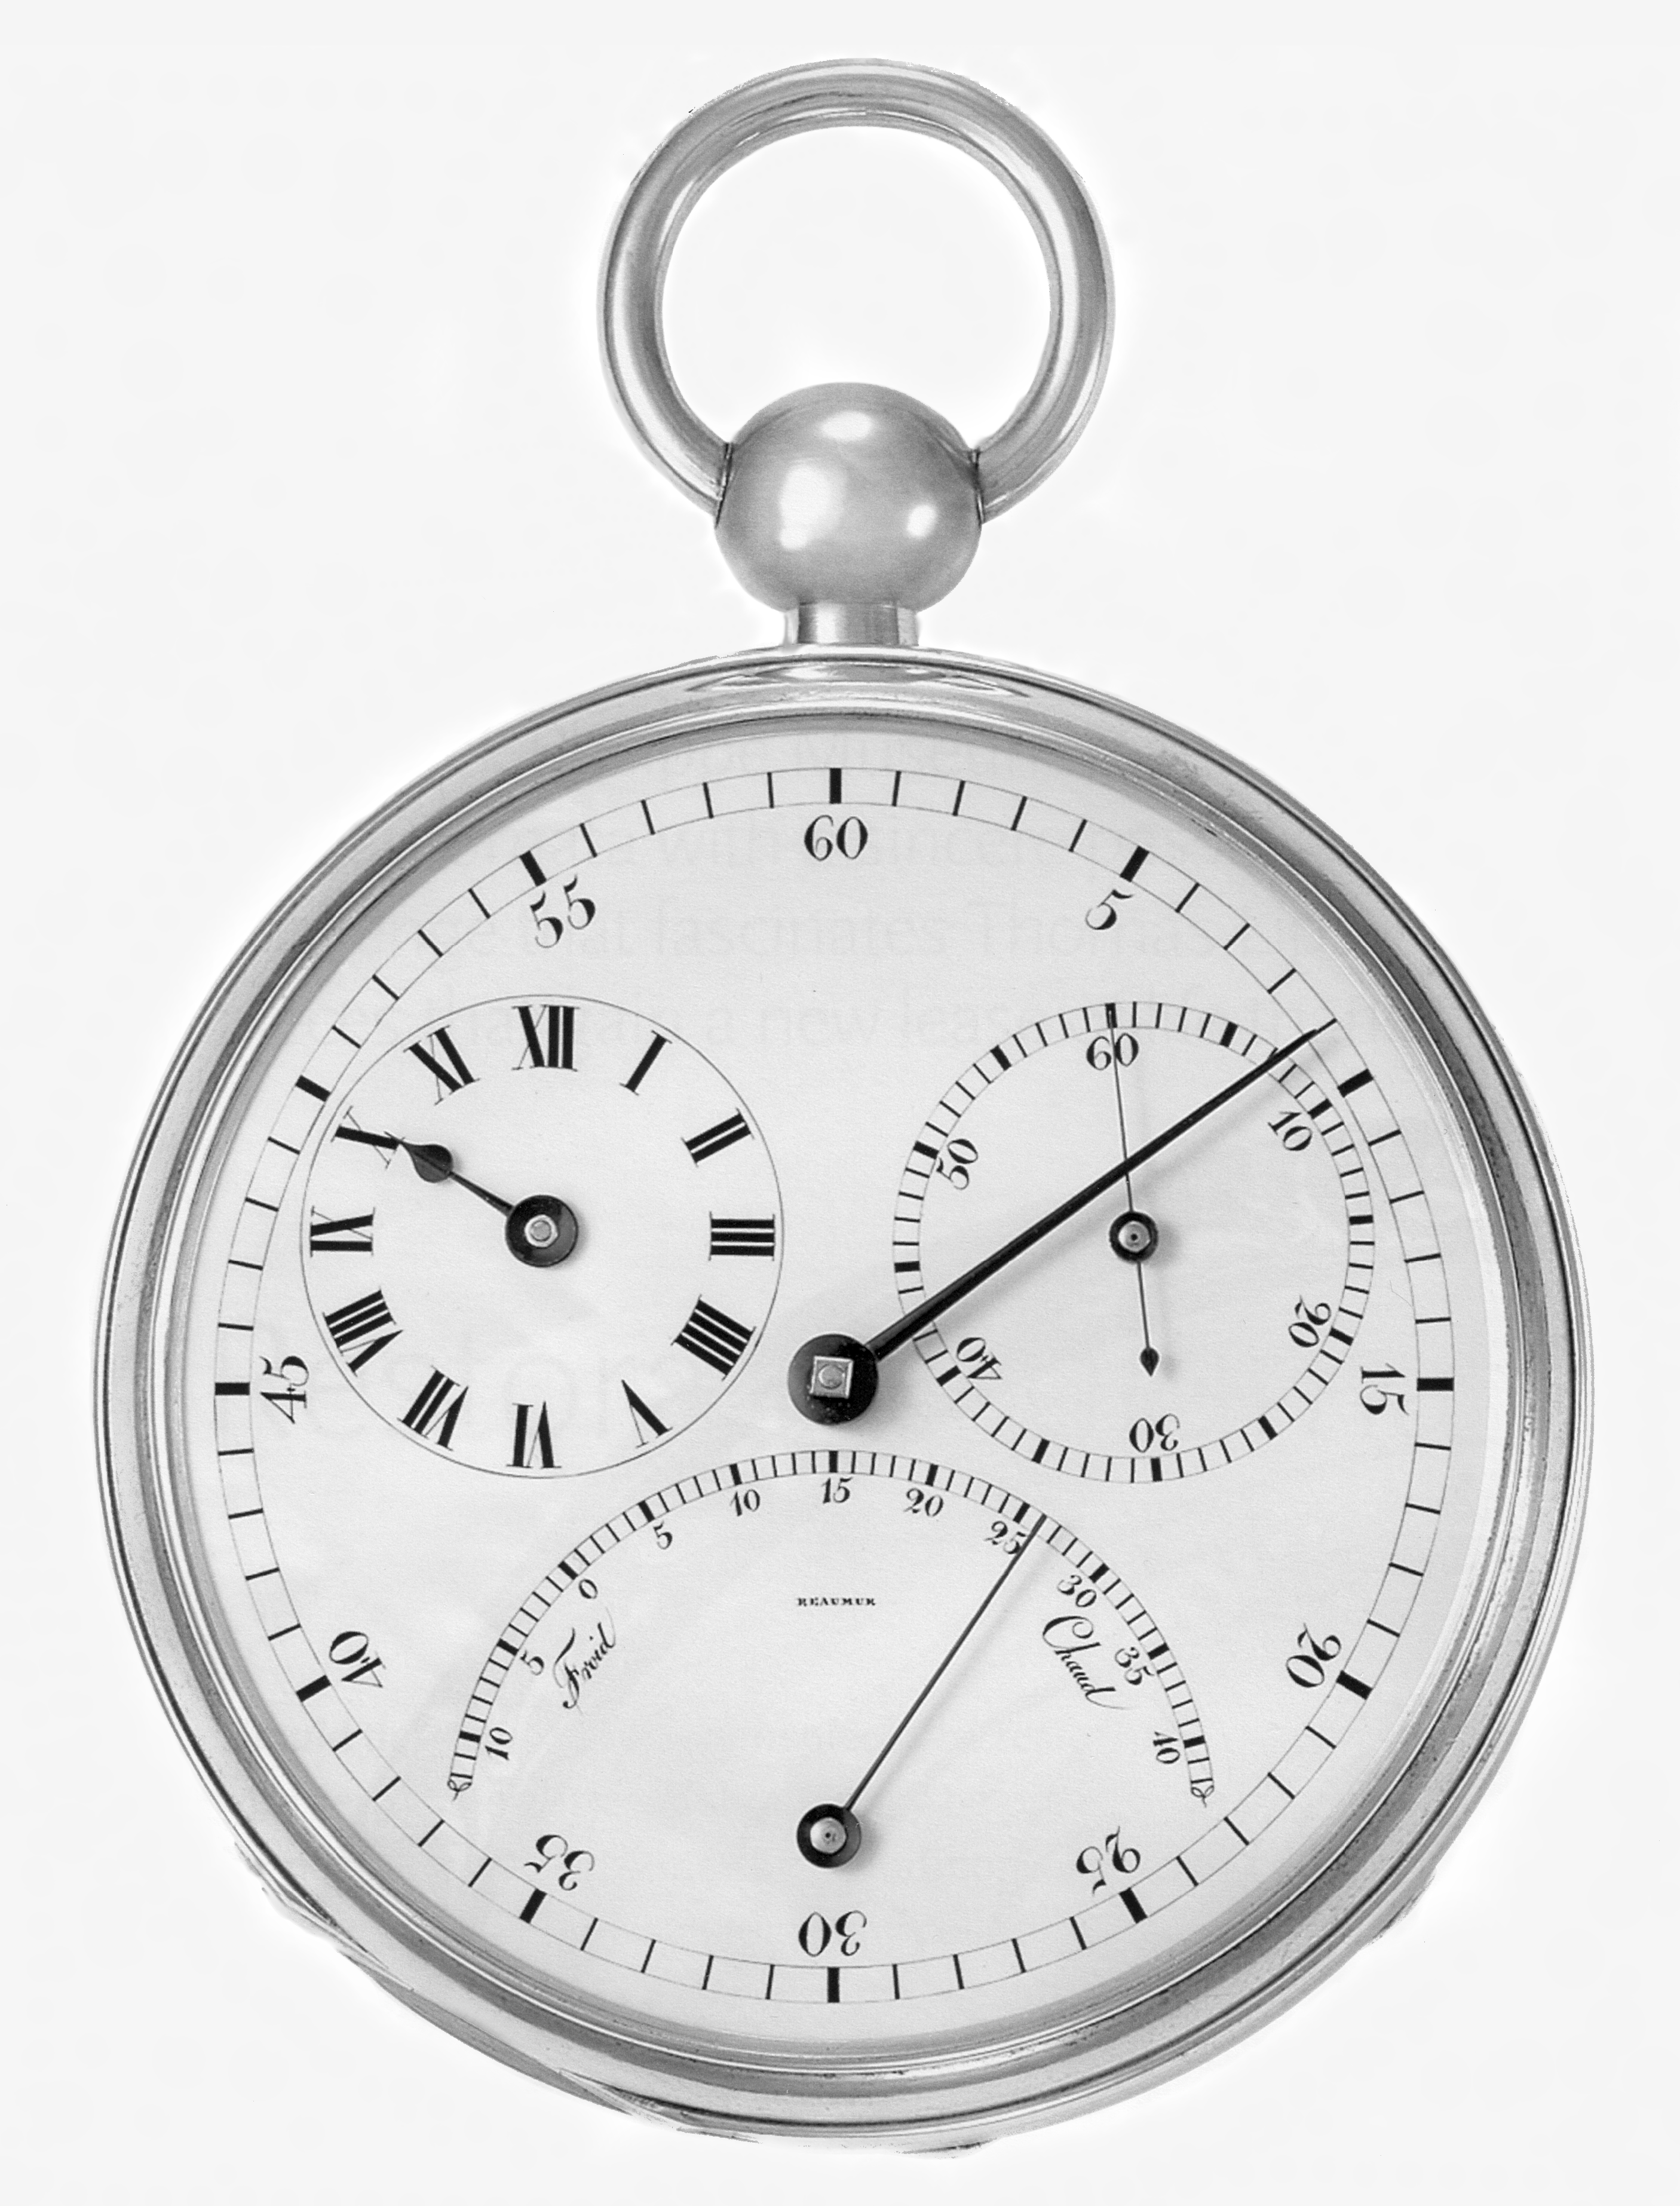
\includegraphics[width=.25\textwidth]{../lab1ex1/clockhigh.png}
\caption{original image}
\end{figure}
\item
When you shrink the original image pixel information is lost, since only every tenth pixel is used 
for the new image. When zooming in, the information can not be retrieved, since the new image only contains
the samples of every tenth pixel.

\end{enumerate}



\exercise{Histogram equalization}
\begin{enumerate}
\item 
The histogram is created by iterating over all pixels and keeping of the number 
of occurences of each gray value.
This 1D array is then plotted.
\lstinputlisting{../lab1ex2/IPhistogram.m}
\item
The function uses the histogram of the former exercise.
It can be given as an argument or is created by the function itself.
Then a cumulative histogram is created. The histogram is then normalised for the number of pixels.
Then a new image is created by iterating over all the pixels in the original image.
For each pixel, the value is looked up in the cumulative histrogram and then multiplied by
256 to acquire the new gray levels.
\lstinputlisting{../lab1ex2/IPhisteq.m}
\item
\begin{figure}[H]
\centering
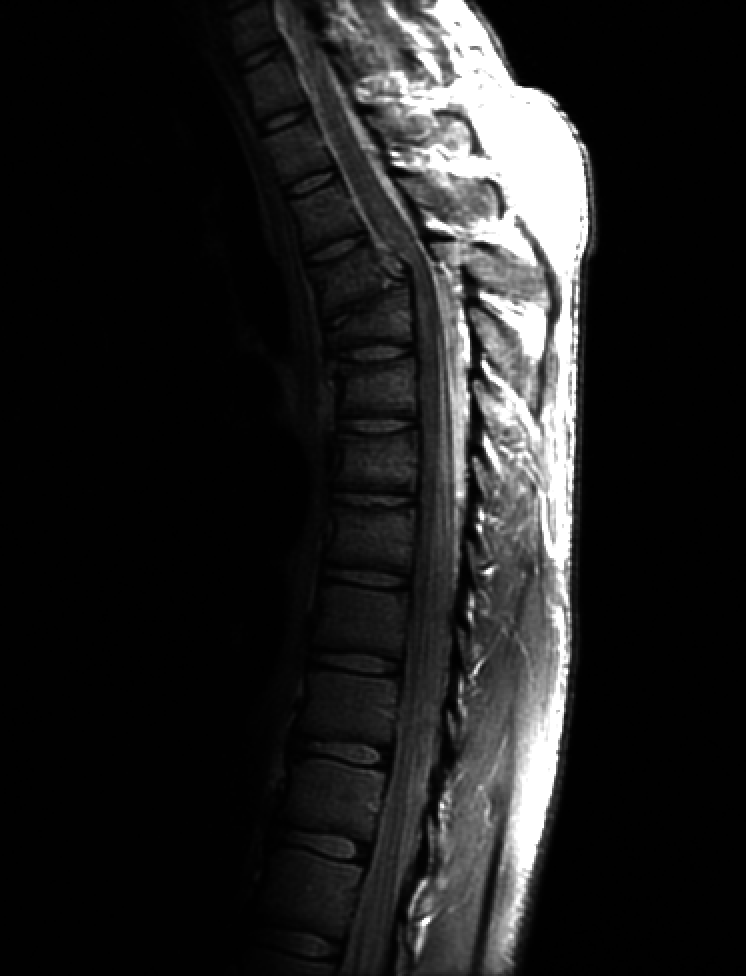
\includegraphics[width=.5\textwidth]{../lab1ex2/fracturedspine.png}
\caption{Original image}
\end{figure}
\begin{figure}[H]
\centering
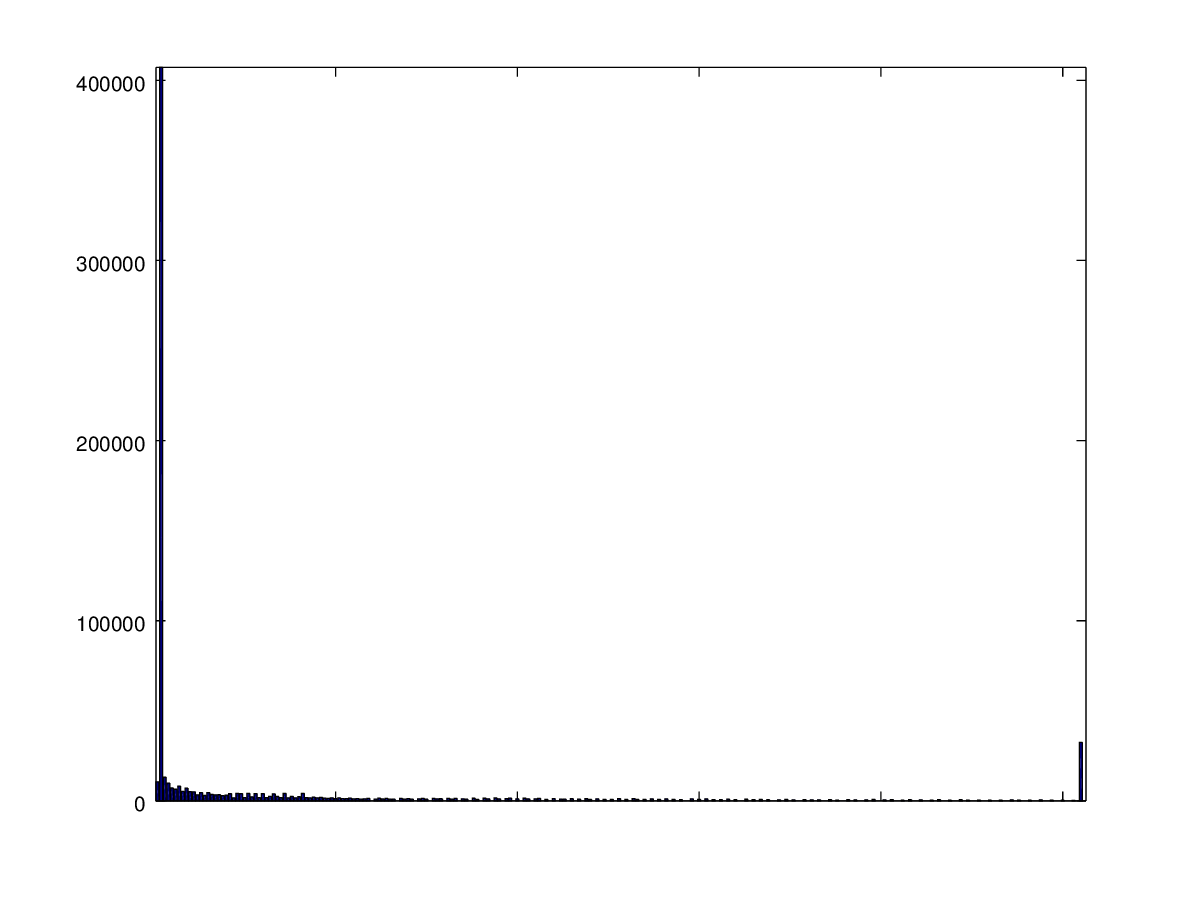
\includegraphics[width=.75\textwidth]{../lab1ex2/histogram1.png}
\caption{Histogram of the original image}
\end{figure}


\begin{figure}[H]
\centering
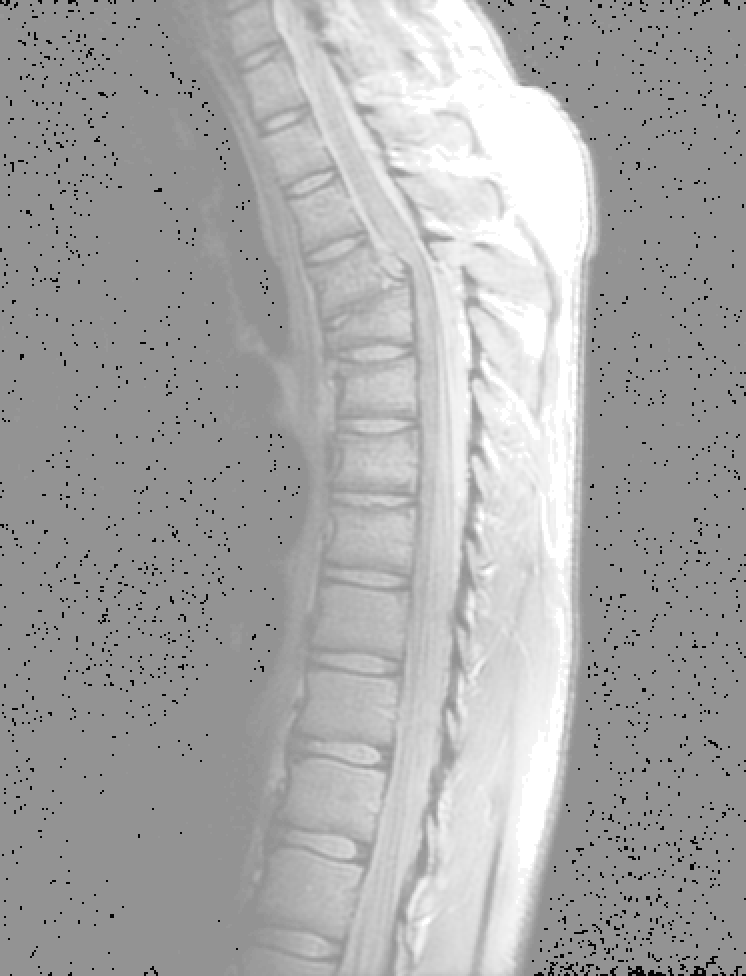
\includegraphics[width=.5\textwidth]{../lab1ex2/result.png}
\caption{Image after histogram equalization}
\end{figure}

\begin{figure}[H]
\centering
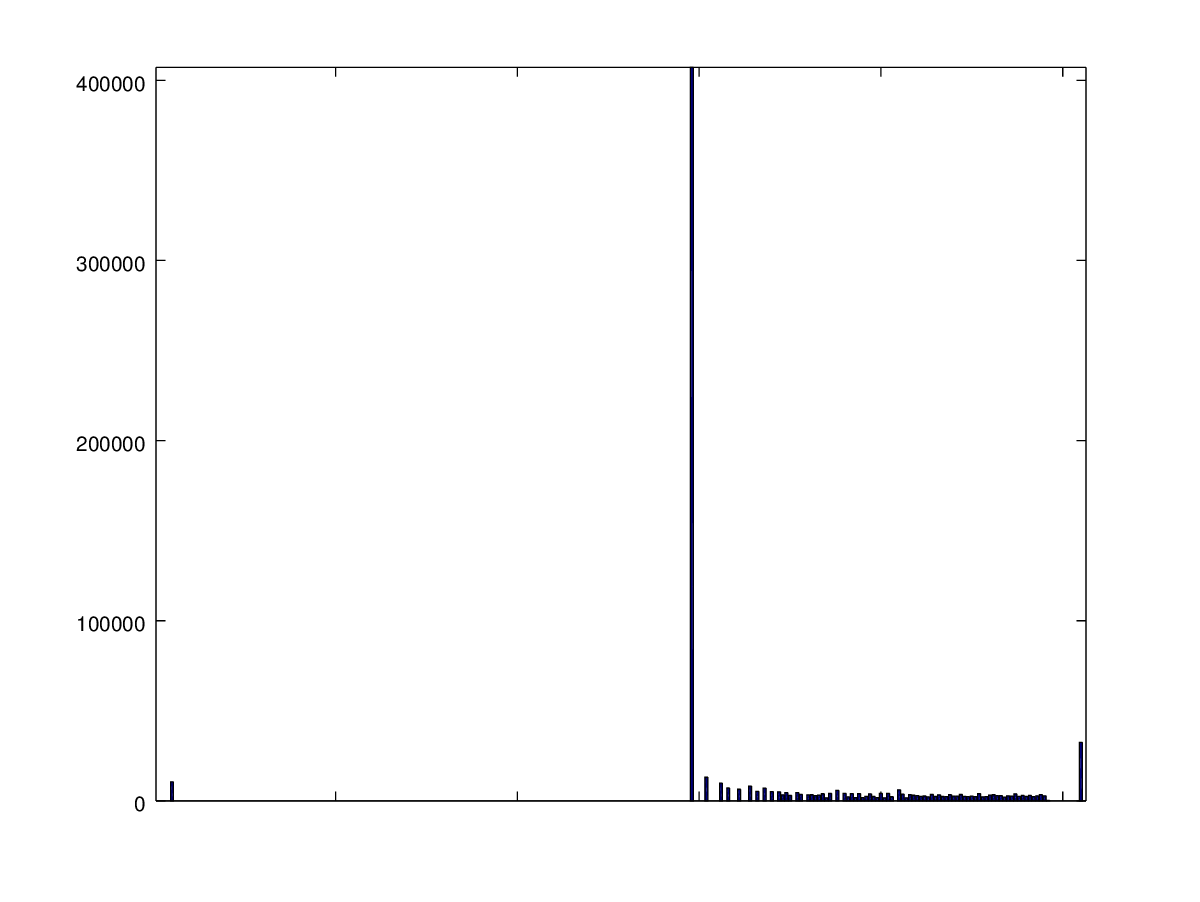
\includegraphics[width=.75\textwidth]{../lab1ex2/histogram2.png}
\caption{Histogram of the resulting image}
\end{figure}

The resulting image after histogram equalization has a wider spread of gray values,
by making each gray level occur more equally.
This allows for more contrast in the hard to see dark values on the leftside of the spine.
The large peak in the centre of the histogram is the result of the large peak in the black values.
This cannot be solved by the histogram equalization, because these values are all the same.

\item
%Why does it not work appyling it again.
Applying the histogram equalization again would have no effect.
Since the histogram after one pass of the algorithm already should make the histogram as
flat as possible.
\end{enumerate}

\exercise{Spatial filtering}
\begin{enumerate}
\item
The algorithm is based on the algorithm shown in the slides for applying a uniform mask.
First, 8 images are created from the original image by shifting rows and columns in the 8 neighborhood.
Then each part of the mask is applied seperately on each of these images in such that
the each part of the mask is applied to the right (shifted) image.
These values are then summed to achieve correlation of the image with the mask.
\lstinputlisting{../lab1ex3/IPfilter.m}
\item
This function uses the IPfilter function from the previous step and the given equations. It applies the vertical
and horizontal Sobel mask. The resulting image is retrieved by adding these togehter after taking
the absolute value.
\lstinputlisting{../lab1ex3/IPSobel.m}

\begin{figure}[H]
\centering
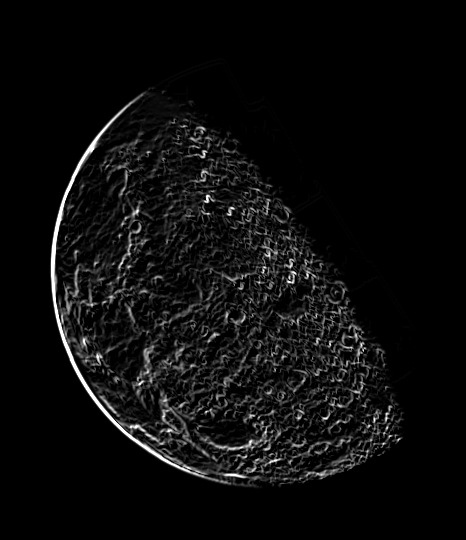
\includegraphics[width=.75\textwidth]{../lab1ex3/blurrymoonsobel.png}
\caption{The result of the application of the IPSobel function to blurrymoon.tif}
\end{figure}

\end{enumerate}

\section*{Task distribution}

\begin{table}[H]
\begin{tabular}{ccccc}
ex1 & design & implementation & answers questions & writing report \\
\hline
Klaas & 80\% & 80\% & 50\% & 50\% \\
\hline
Jan & 20\% & 20\% & 50\% & 50\% \\
\end{tabular}
\end{table}

\begin{table}[H]
\begin{tabular}{ccccc}
ex2 & design & implementation & answers questions & writing report \\
\hline
Klaas & 80\% & 80\% & 50\% & 50\% \\
\hline
Jan & 20\% & 20\% & 50\% & 50\% \\
\end{tabular}
\end{table}

\begin{table}[H]
\begin{tabular}{ccccc}
ex3 & design & implementation & answers questions & writing report \\
\hline
Klaas & 20\% & 20\% & 50\% & 50\% \\
\hline
Jan & 80\% & 80\% & 50\% & 50\% \\
\end{tabular}
\end{table}

\end{document}
